% statistics_and_probability:x12 GDC:YES
\begin{question}
  \hspace*{\fill} [Note maximale: 6]\par
  \noindent Le tableau suivant montre le poids moyen, y kg , d’enfants âgés de x ans.\par
  \medskip
  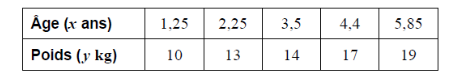
\includegraphics[scale=0.5]{tableau_age_poids}\par
  \noindent La relation entre les variables est modélisée par la droite de régression d’équation $y = ax + b$\par
  (a)\par
  \medskip
  \hspace{1em}(i)  Trouvez la valeur de a et celle de b.\par
  \medskip
  \hspace{1em}(ii) Écrivez le coefficient de corrélation.\hspace*{\fill} [4]\par
  \bigskip
  (b) Utilisez votre équation pour estimer le poids moyen d’un enfant âgé de 1,95 an.\hspace*{\fill} [2]\par
  
\end{question}

